\documentclass[12pt,onecolumn]{article}
% ==================== PREÁMBULO ====================
% Archivo para centralizar la configuración de paquetes y estilos del documento.

% ----- IDIOMA Y CODIFICACIÓN -----
\usepackage[T1]{fontenc}
\usepackage[utf8]{inputenc}
\usepackage[spanish,english]{babel}

% ----- GEOMETRÍA Y TIPOGRAFÍA -----
\usepackage[letterpaper,margin=2.2cm]{geometry}
\usepackage{mathptmx} % Fuente tipo Times para formato académico/IEEE
\usepackage{setspace}
\setstretch{1.05}
\usepackage{parskip}
\usepackage{enumitem}
\setlist{nosep}

% ----- PAQUETES MATEMÁTICOS -----
\usepackage{amsmath,amssymb,amsfonts}

% ----- FIGURAS Y GRÁFICOS -----
\usepackage{graphicx}
\usepackage{xcolor}
\usepackage{float}
\usepackage{tikz}
\usetikzlibrary{mindmap, positioning, arrows.meta, shapes.geometric}

% ----- TABLAS -----
\usepackage{booktabs}
\usepackage{tabularx}
\usepackage{array}
\usepackage{multirow}
\usepackage{multicol}
\usepackage{threeparttable}
\usepackage{longtable}

% ----- BIBLIOGRAFÍA Y REFERENCIAS -----
\usepackage[numbers]{natbib}
\usepackage{xurl}      % Permite cortar enlaces largos en varias líneas
\usepackage{url}
\usepackage{hyperref}
\hypersetup{
  colorlinks=true,
  linkcolor=black,
  citecolor=black,
  urlcolor=blue,
  breaklinks=true
}
\Urlmuskip=0mu plus 2mu

% ----- CÓDIGO Y COMANDOS -----
\usepackage{listings}
\lstdefinestyle{terminal}{
  basicstyle=\ttfamily\small,
  frame=single,
  breaklines=true,
  columns=fullflexible,
  backgroundcolor=\color{gray!8},
  rulecolor=\color{gray!45},
  xleftmargin=0.5em,
  xrightmargin=0.5em
}
\lstset{style=terminal}

% ----- AJUSTES TIPOGRÁFICOS -----
\usepackage{etoolbox}
\hbadness=10000
\vbadness=10000
\tolerance=10000

% ----- COMANDOS PROPIOS -----
\newcommand{\evidencia}[2]{%
\begin{figure}[H]
\centering
\fbox{\begin{minipage}[c][0.18\textheight][c]{0.92\textwidth}
\centering
\textbf{#1}\\[0.4em]
\small Inserte aquí el recorte de pantalla: \texttt{#2}
\end{minipage}}
\caption{#1}
\end{figure}}


\begin{document}

\begin{center}

{\Large \textbf{Taller evaluable: creación de repositorio en GitHub desde Visual Studio Code}}\\
{\normalsize Sistemas Embebidos / Herramientas de desarrollo colaborativo}\\[0.5em]
\end{center}

\noindent\textbf{Nombre del estudiante:} \rule{8cm}{0.4pt}\hfill
\textbf{Fecha:} \rule{3cm}{0.4pt}

\section*{1. Propósito del taller}
El propósito de este taller es que el estudiante evidencie la creación de un primer proyecto local en Visual Studio Code, la inicialización del repositorio con Git y la publicación del proyecto en una cuenta personal de GitHub. El entregable principal será este archivo en formato PDF, con enlaces y recortes de pantalla.

\section*{2. Software y paquetes requeridos}
Antes de iniciar, verifique que el computador tenga instaladas las siguientes herramientas. Copie los enlaces en el navegador y realice la instalación cuando sea necesario.

\begin{table}[H]
\centering
\small
\begin{tabularx}{\textwidth}{p{3.2cm}X}
\toprule
\textbf{Herramienta} & \textbf{Enlace recomendado} \\
\midrule
Visual Studio Code & \url{https://code.visualstudio.com/} \\
Git para Windows & \url{https://git-scm.com/downloads/win} \\
Cuenta de GitHub & \url{https://github.com/} \\
Extensión GitHub Pull Requests and Issues & \url{https://marketplace.visualstudio.com/items?itemName=GitHub.vscode-pull-request-github} \\
Extensión C/C++ de Microsoft & \url{https://marketplace.visualstudio.com/items?itemName=ms-vscode.cpptools} \\
PlatformIO IDE, si el proyecto usa ESP32 & \url{https://platformio.org/install/ide?install=vscode} \\
\bottomrule
\end{tabularx}
\end{table}

\textbf{Nota:} Para evitar problemas con los enlaces en el documento, este archivo utiliza los paquetes \texttt{hyperref}, \texttt{url} y \texttt{xurl}. El estudiante debe pegar los enlaces completos usando \verb|\url{...}|.

\section*{3. Estructura mínima del proyecto en Overleaf}
El estudiante debe cargar este documento en Overleaf conservando la siguiente estructura de carpetas:

\begin{lstlisting}
main.tex
preamble.tex
reference.bib
/images
/images/evidencias
/section
/tables
\end{lstlisting}

Los recortes de pantalla deben guardarse dentro de la carpeta:

\begin{lstlisting}
images/evidencias/
\end{lstlisting}

\section*{4. Actividad práctica}
Realice las siguientes acciones. No se calificará solamente que el repositorio exista; se calificará que el estudiante pueda demostrar el proceso mediante evidencias.

\subsection*{4.1 Crear el proyecto local}
Abra Visual Studio Code, cree una carpeta de trabajo y genere al menos un archivo de código. Puede usar un archivo \texttt{main.cpp}, \texttt{main.py} o similar, de acuerdo con la práctica del curso.

\begin{figure}[H]
\centering
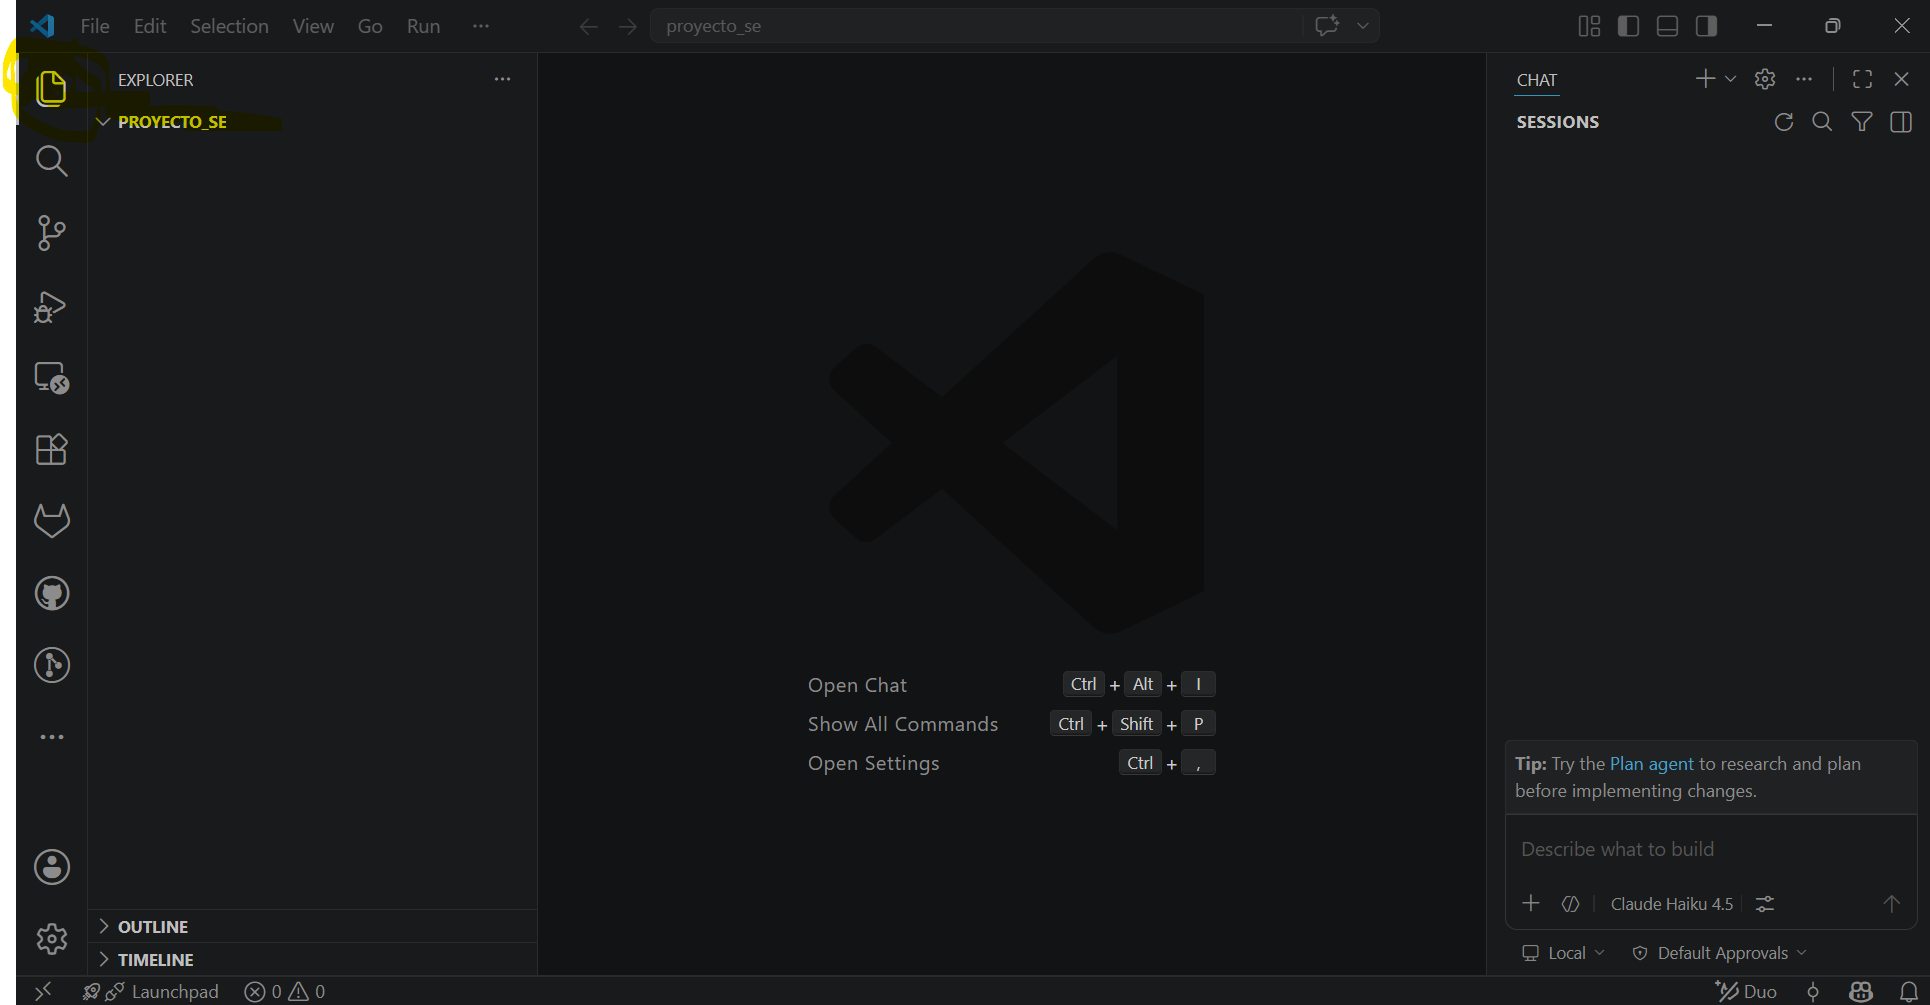
\includegraphics[width=0.88\textwidth]{images/ventana_vscode.png}
\caption{Ejemplo de proyecto abierto en Visual Studio Code.}
\end{figure}

\begin{figure}[H]
\centering
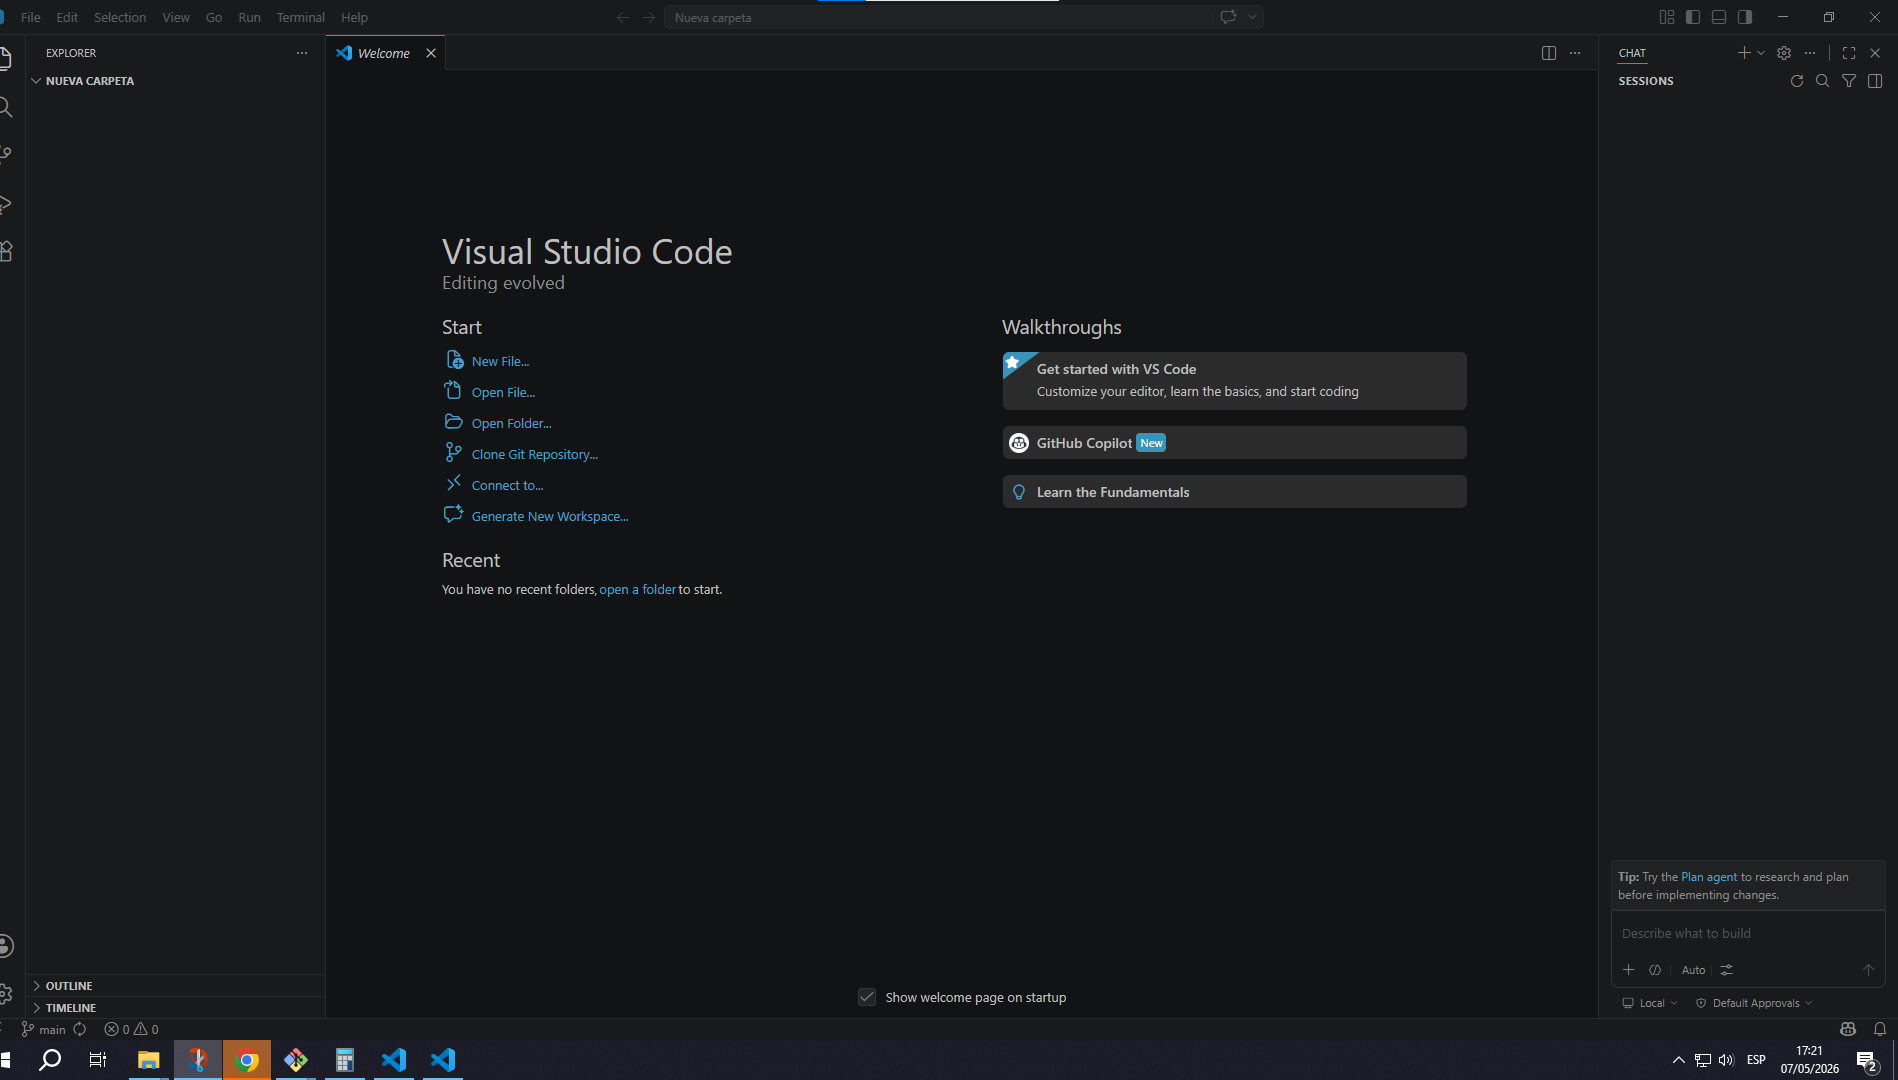
\includegraphics[width=0.88\textwidth]{images/evidencia1.png}
\caption{Evidencia 1: proyecto local creado en Visual Studio Code}
\end{figure}

\subsection*{4.2 Verificar Git desde la terminal de VS Code}
Abra la terminal integrada de Visual Studio Code y ejecute:

\begin{lstlisting}
git --version
\end{lstlisting}

\begin{figure}[H]
\centering
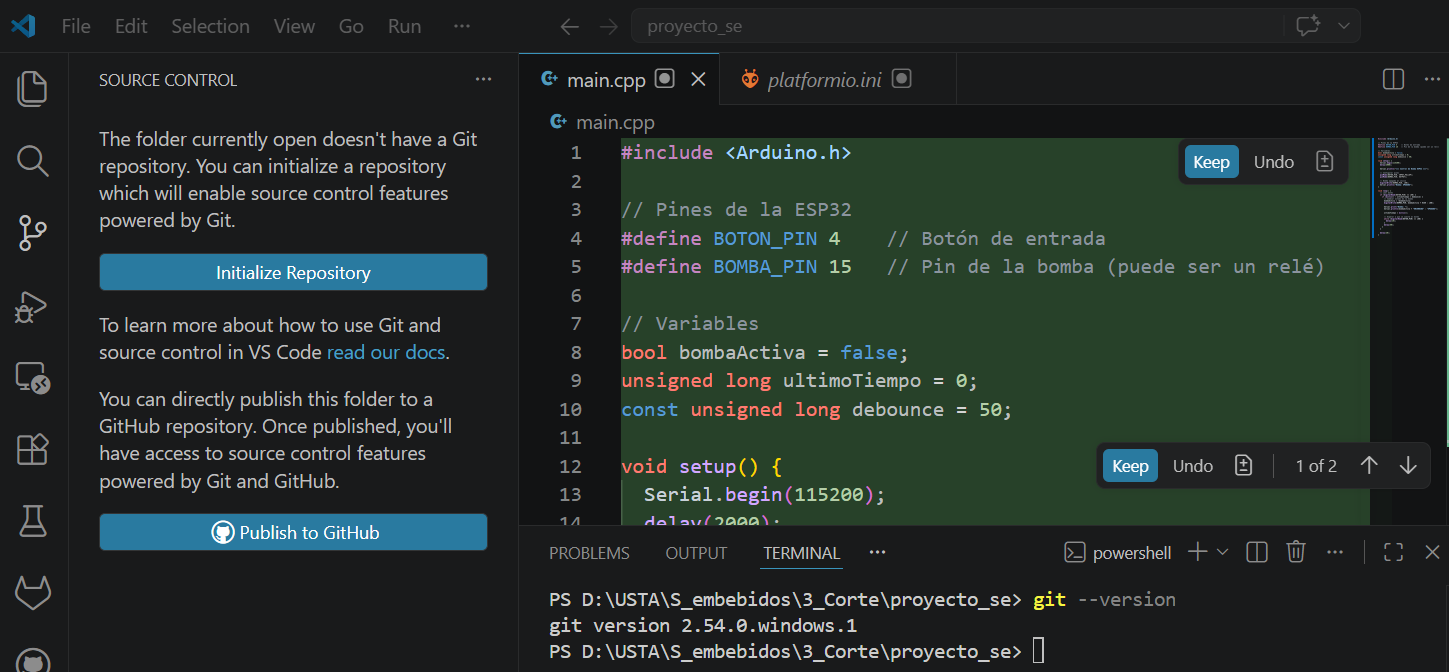
\includegraphics[width=0.88\textwidth]{images/git_version.png}
\caption{Ejemplo de verificación de Git desde la terminal de Visual Studio Code.}
\label{git_ver}
\end{figure}

\begin{figure}[H]
\centering
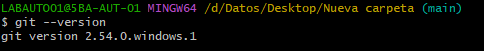
\includegraphics[width=0.88\textwidth]{images/evidencia2.png}
\caption{Evidencia 2: versión de Git instalada}
\end{figure}

\subsection*{4.3 Inicializar el repositorio local y realizar el primer commit}
Desde la terminal integrada de VS Code, ejecute los comandos en el siguiente orden:

\begin{lstlisting}
git init
git status
git add .
git commit -m "inicio proyecto"
git branch -M main
\end{lstlisting}

\textbf{Importante:} si se intenta hacer \texttt{git commit} sin ejecutar primero \texttt{git add .}, Git mostrará que no hay archivos agregados para confirmar. El comando \texttt{git add .} prepara todos los archivos del proyecto para el commit.

\begin{figure}[H]
\centering
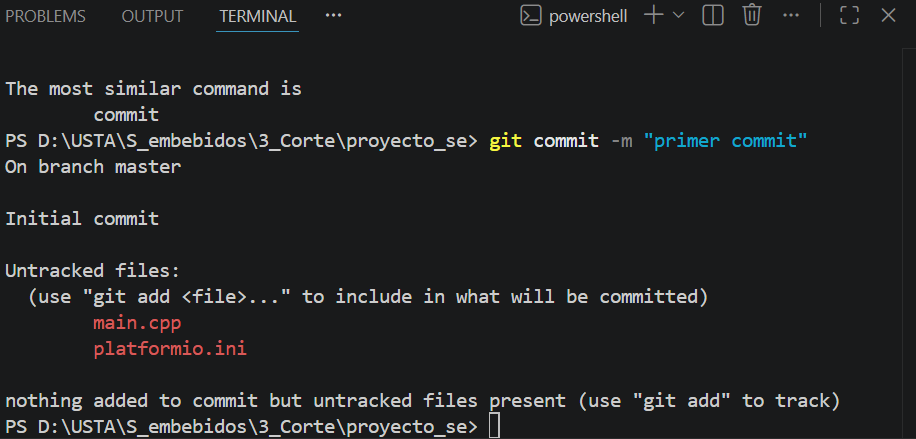
\includegraphics[width=0.88\textwidth]{images/primer_commit.png}
\caption{Ejemplo del primer commit realizado desde la terminal.}
\end{figure}

\begin{figure}[H]
\centering
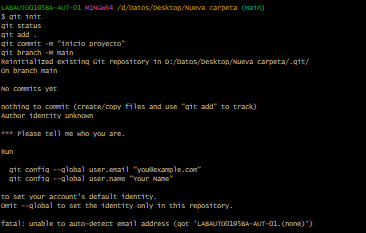
\includegraphics[width=0.88\textwidth]{images/evidencia3.png}
\caption{Evidencia 3: primer commit del proyecto}
\end{figure}

\subsection*{4.4 Crear el repositorio en GitHub}
Ingrese a GitHub, cree un nuevo repositorio y copie la URL HTTPS del repositorio. No agregue archivos iniciales si desea cargar el proyecto desde la terminal local.

\begin{figure}[H]
\centering
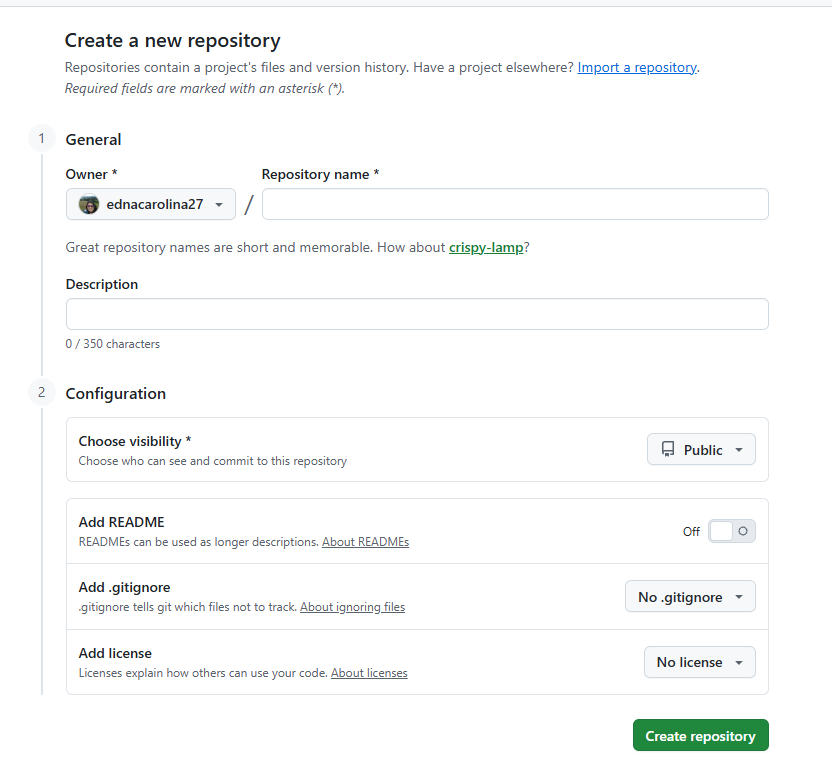
\includegraphics[width=0.82\textwidth]{images/crear_nuevo_Rep.png}
\caption{Ejemplo de creación de un nuevo repositorio en GitHub.}
\end{figure}

\begin{figure}[H]
\centering
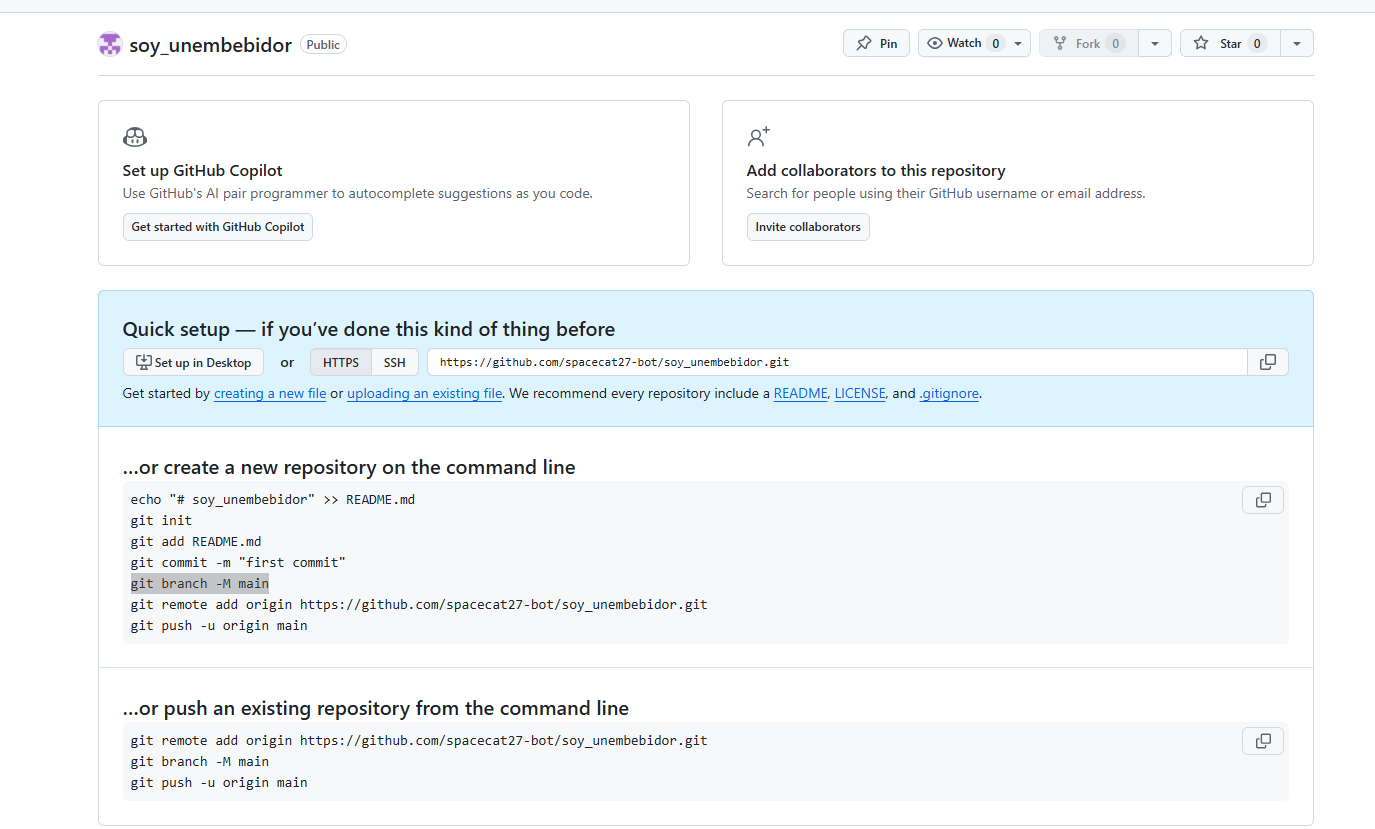
\includegraphics[width=0.88\textwidth]{images/evidencia4.png}
\caption{Evidencia 4: repositorio creado en GitHub}
\end{figure}

\subsection*{4.5 Conectar el repositorio local con GitHub y cargar el proyecto}
Use la URL HTTPS de su repositorio y ejecute:

\begin{lstlisting}
git remote add origin https://github.com/USUARIO/NOMBRE_REPOSITORIO.git
git push -u origin main
\end{lstlisting}

Si el remoto ya existe, use:

\begin{lstlisting}
git remote set-url origin https://github.com/USUARIO/NOMBRE_REPOSITORIO.git
git push -u origin main
\end{lstlisting}

\begin{figure}[H]
\centering
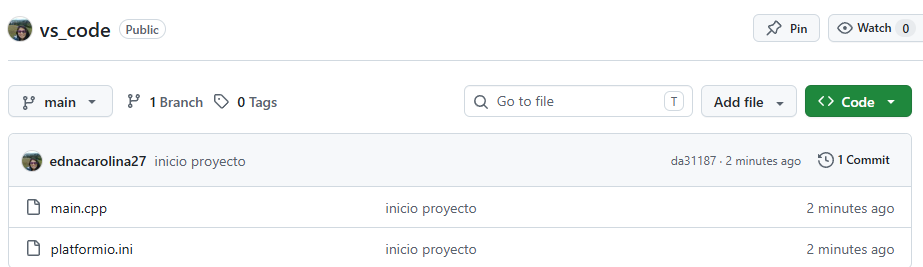
\includegraphics[width=0.88\textwidth]{images/primer_proyec_creado.png}
\caption{Ejemplo de proyecto cargado correctamente en GitHub.}
\end{figure}

\begin{figure}[H]
\centering
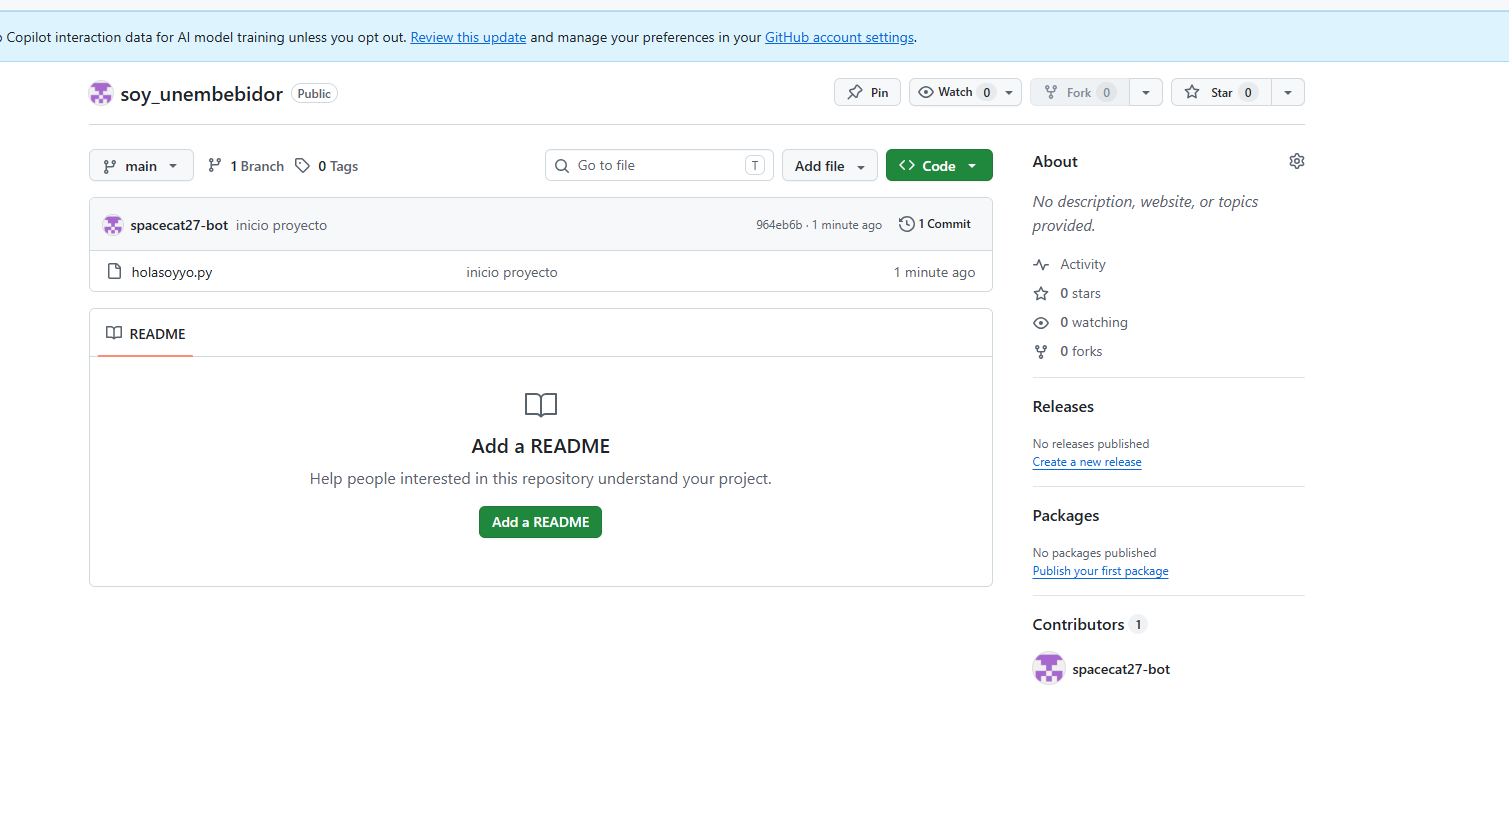
\includegraphics[width=0.88\textwidth]{images/evidencia5.png}
\caption{Evidencia 5: archivos cargados en GitHub}
\end{figure}

\section*{5. Enlaces obligatorios del entregable}
Diligencie los siguientes campos usando enlaces completos.

\begin{enumerate}
    \item \textbf{Enlace del repositorio en GitHub:} \\
    \url{PEGAR_AQUI_EL_LINK_DEL_REPOSITORIO}

    \item \textbf{Enlace al archivo principal del proyecto, por ejemplo \texttt{main.cpp}:} \\
    \url{PEGAR_AQUI_EL_LINK_DEL_ARCHIVO_PRINCIPAL}

    \item \textbf{Enlace al perfil de GitHub del estudiante:} \\
    \url{PEGAR_AQUI_EL_LINK_DEL_PERFIL}
\end{enumerate}

\section*{6. Evidencias que deben adjuntarse}
El documento final debe incluir mínimo cinco evidencias en la carpeta \texttt{images/evidencias/}:

\begin{table}[H]
\centering
\small
\begin{tabularx}{\textwidth}{p{0.5cm}X p{6cm}}
\toprule
\textbf{No.} & \textbf{Nombre sugerido} & \textbf{Contenido esperado} \\
\midrule
1 & \texttt{evidencia\_01\_vscode.png} & Carpeta del proyecto abierta en Visual Studio Code y el archivo creado. \\
2 & \texttt{evidencia\_02\_git\_version.png} & Terminal con el comando \texttt{git --version}. \\
3 & \texttt{evidencia\_03\_commit.png} & Terminal con \texttt{git add .}, \texttt{git commit} y \texttt{git branch -M main}. \\
4 & \texttt{evidencia\_04\_repositorio\_github.png} & Repositorio creado en GitHub. \\
5 & \texttt{evidencia\_05\_push\_github.png} & Repositorio en GitHub que muestra los archivos cargados. \\
\bottomrule
\end{tabularx}
\end{table}

\section*{7. Criterios de evaluación}

\begin{table}[H]
\centering
\small
\begin{tabularx}{\textwidth}{Xc}
\toprule
\textbf{Criterio} & \textbf{Valor} \\
\midrule
Instalación y verificación de herramientas: VS Code, Git y cuenta de GitHub. & 20\% \\
Creación del proyecto local y archivo de código inicial. & 20\% \\
Uso correcto de Git: \texttt{init}, \texttt{add}, \texttt{commit}, rama \texttt{main}. & 25\% \\
Publicación del repositorio en GitHub y enlace funcional. & 25\% \\
Orden del documento, evidencias completas y enlaces funcionales. & 10\% \\
\bottomrule
\end{tabularx}
\end{table}

\begin{thebibliography}{00}

\bibitem{vscode}
Microsoft, ``Visual Studio Code,'' 2026. [Online]. Available:
\url{https://code.visualstudio.com/}

\bibitem{git}
Git, ``Git downloads,'' 2026. [Online]. Available:
\url{https://git-scm.com/downloads}

\bibitem{github}
GitHub Docs, ``Set up Git,'' 2026. [Online]. Available:
\url{https://docs.github.com/en/get-started/git-basics/set-up-git}

\bibitem{platformio}
PlatformIO, ``PlatformIO IDE for VSCode,'' 2026. [Online]. Available:
\url{https://platformio.org/install/ide?install=vscode}

\end{thebibliography}

\end{document}